\section{Processi primari}
    \subsection{Fornitura}
        \subsubsection{Scopo}
        Lo scopo del processo di fornitura è di determinare le procedure e le risorse necessarie allo svolgimento del progetto. Le attività di cui si compone sono:
        \begin{itemize}
            \item studio di fattibilità;
            \item contrattazione;
            \item collaudo.
        \end{itemize}
        La corretta implementazione del processo deve:
        \begin{itemize}
            \item decidere il progetto da svolgere;
            \item fissare gli obiettivi per la contrattazione.
        \end{itemize}
        \subsubsection{Studio di fattibilità}
            \paragraph{Scopo}
            Individuare gli aspetti fondamentali dei progetti proposti, tramite lo studio dei \glo{Capitolato}{capitolati} ed il confronto tra i membri del \glo{Gruppo}{gruppo}.
            \paragraph{Discussione e scelta del capitolato}
            Il \responsabilediprogetto{} ha il compito di organizzare gli incontri del gruppo necessari ad analizzare i capitolati proposti.
            \paragraph{Struttura studio di fattibilità}
            Il documento creato dagli \analisti{} per ogni capitolato deve rispettare i seguenti punti:
            \begin{itemize}
                \item \textbf{descrizione:} descrizione del prodotto richiesto dal capitolato;
                \item \textbf{dominio applicativo:} ambito di utilizzo del prodotto;
                \item \textbf{dominio tecnologico:} tecnologie richieste per lo sviluppo del progetto;
                \item \textbf{criticità:} individuazione di punti critici e possibili problematiche che potrebbero sorgere durante lo svolgimento del progetto;
                \item \textbf{valutazione finale:} considerazioni finali sulla scelta di accettare o meno il capitolato preso in esame.
            \end{itemize}
        \subsubsection{Contrattazione}
            \paragraph{Scopo}
            Presentare una proposta in risposta al capitolato del proponente.
            \paragraph{Preparazione della proposta}
            Il gruppo deve redigere e consegnare i seguenti documenti:
            \begin{itemize}
                \item \ndp;
                \item \sdf;
                \item \adr;
                \item \pdp;
                \item \pdq.
            \end{itemize}
            Verrà inoltre fornita in allegato la \ldp{} del gruppo. Si veda la sezione \ref{sec:classDoc} per maggiori informazioni sulla gestione dei documenti.
        \subsubsection{Consegna}
	        \paragraph{Scopo}
	        Preparare il materiale richiesto per la \revacc.
	        \paragraph{Preparazione della consegna}
	        Deve essere preparato un supporto ottico (CD/DVD) contente:
		    \begin{itemize}
		    	\item la \ldp{} del gruppo per la \revacc;
		    	\item le versioni finali di tutti i documenti;
		    	\item il prodotto finale realizzato comprensivo di:
			    	\begin{itemize}
			    		\item codice sorgente;
			    		\item eventuali unità di compilazione e installazione;
			    		\item istruzioni per l'uso.
			    	\end{itemize}
		    \end{itemize}
	        Il \responsabilediprogetto{} ha il compito di contattare il committente per richiedere un appuntamento per consegnare il supporto preparato.
	        \paragraph{Consegna}
	        Il \responsabilediprogetto{} deve contattare il proponente per accordarsi sulle modalità di consegna del prodotto finale.
		\subsubsection{Procedure}
			\paragraph{Primo contatto con il proponente}
			Il primo contatto con il proponente da parte del gruppo \zephyrus{} deve essere effettuato da parte del \responsabilediprogetto{}. L'oggetto del messaggio deve contenere la sigla del progetto; il messaggio deve essere realizzato secondo la seguente struttura:
			\bigskip
				\begin{verbatim}
				Spett.le Nome Azienda, 
				alla cortese attenzione del CEO/Responsabile Nome Cognome;
				
				... corpo del messaggio ...
				
				Vi ringraziamo e speriamo di poterci incontrare presto di persona.
				
				Cordiali saluti,
				Zephyrus.
				\end{verbatim}
			\paragraph{Consegna materiale per revisione di avanzamento}
			La consegna del materiale prodotto deve rispettare i vincoli temporali descritti al seguente indirizzo:
			\begin{center}
				\url{http://www.math.unipd.it/~tullio/IS-1/2016/}
			\end{center}
			L'invio del materiale deve essere gestito nel seguente modo:
			\begin{enumerate}
				\item creare una cartella compressa contenente tutti e soli i documenti inerenti la consegna in formato pdf. Il nome della cartella sarà: \texttt{Zephyrus-XX.zip} dove al posto di XX sarà presente il codice identificativo della revisione di avanzamento;
				\item caricarla sullo spazio web del gruppo, disponibile al seguente indirizzo:
				\begin{center}
% 	\href{https://s311.altervista.org/lf.pl?sid=e085c1d3474a6fb0a08d56cafc9e60e3https://s311.altervista.org/lf.pl?sid=e085c1d3474a6fb0a08d56cafc9e60e3}{Altervista Zephyrus}
					\href{http://zephyrusar.altervista.org/}{Altervista Zephyrus}
				\end{center}
			\item contattare con l'email del gruppo, il committente all'indirizzo \url{tullio.vardanega@math.unipd.it} e allegare il link al file precedentemente caricato su Altervista.
			\end{enumerate}
    \subsection{Sviluppo}
        \subsubsection{Scopo}
	        Il processo di sviluppo contiene le attività necessarie a produrre il prodotto software richiesto. In accordo con lo standard \glo{ISO}{ISO}/\glo{IEC}{IEC} (\ref{sec:isoiec}), preso come riferimento, si è deciso di istanziare le seguenti attività:
        \begin{itemize}
            \item analisi dei requisiti;
            \item progettazione;
            \item codifica.
        \end{itemize}
        La corretta implementazione del processo deve:
        \begin{itemize}
            \item fissare gli obiettivi di sviluppo;
            \item fissare i vincoli tecnologici;
            \item realizzare un prodotto finale che soddisfi i test di accettazione e che sia conforme alle richieste del proponente.
        \end{itemize}
        \subsubsection{Analisi dei requisiti}
            \paragraph{Scopo}
            Individuare i requisiti del progetto tramite lo studio del capitolato ed incontri con il proponente. Individuare i test di sistema. Il risultato deve essere presentato nel documento formale \adr{} che deve contenere la lista dei casi d'uso e dei requisti.
            \paragraph{Classificazione dei casi d'uso}
            I casi d'uso individuati devono essere classificati secondo la seguente notazione:
            \begin{center}
            UC[Codice padre].[Codice identificativo]
            \end{center}
            dove:
            \begin{itemize}
                \item \textbf{codice padre:} indica il codice numerico in forma gerarchica del caso d'uso da cui deriva, viene omesso se non identificabile;
                \item \textbf{codice identificativo:} indica il codice numerico del caso d'uso.
            \end{itemize}
            Per ogni caso d'uso bisogna indicare:
            \begin{itemize}
                \item \textbf{titolo:} titolo riassuntivo dell'operazione che il caso d'uso modella;
                \item \textbf{attori:} elenco attori coinvolti;
                \item \textbf{descrizione:} concisa e meno ambigua possibile;
                \item \textbf{pre-condizione:} condizioni sempre vere riferite allo stato del sistema che abilitano lo svolgimento del caso d'uso;
                \item \textbf{post-condizione:} condizioni sempre vere riferite allo stato del sistema dopo lo svolgimento del caso d'uso;
                \item \textbf{scenario principali:} ordine con cui vengono eseguiti i casi d'uso figli;
                \item \textbf{scenari alternativi:} possibili scenari alternativi del caso d'uso;
                \item \textbf{estensioni:} spiegazione di tutte le estensioni, se presenti;
                \item \textbf{inclusioni:} spiegazione di tutte le inclusioni, se presenti;
                \item \textbf{generalizzazioni:} spiegazione di tutte le generalizzazioni, se presenti.
            \end{itemize}

            \paragraph{Classificazione dei requisiti}
            I requisiti individuati devono essere classificati secondo la seguente notazione:
            \begin{center}
            R[Importanza][Tipologia][Codice]
            \end{center}
            dove:
            \begin{itemize}
                \item \textbf{importanza:} può assumere questi valori:
                \begin{itemize}
                    \item \textbf{O:} indica un requisito obbligatorio;
                    \item \textbf{D:} indica un requisito desiderabile;
                    \item \textbf{F:} indica un requisito opzionale (facoltativo).
                \end{itemize}
                \item \textbf{tipologia:} può assumere questi valori:
                \begin{itemize}
                    \item \textbf{F:} indica un requisito funzionale;
                    \item \textbf{Q:} indica un requisito di qualità;
                    \item \textbf{P:} indica un requisito prestazionale;
                    \item \textbf{V:} indica un requisito di vincolo.
                \end{itemize}
                \item \textbf{codice:} codice numerico che identifica il requisito, deve essere univoco ed indicato in forma gerarchica, da sinistra a destra, nella notazione X.Y.Z.
            \end{itemize}
            Per ogni requisito bisogna inoltre indicare:
            \begin{itemize}
                \item \textbf{descrizione:} concisa e meno ambigua possibile;
                \item \textbf{fonte:} l'origine dei requisiti deve essere una delle seguenti:
                \begin{itemize}
                    \item \textbf{capitolato:} derivato direttamente dal testo del capitolato;
                    \item \textbf{interno:} deriva da discussioni interne al gruppo;
                    \item \textbf{verbale:} deriva da un verbale steso in seguito ad un incontro con il proponente. Deve essere indicato il nome del verbale a cui si riferisce;
                    \item \textbf{casi d'uso:} deriva da uno o più casi d'uso. Deve essere indicato il codice identificativo dei casi d'uso a cui si riferisce.
                \end{itemize}
            \end{itemize}
            \paragraph{Diagrammi UML} \label{sec:astahStyle}
                I diagrammi \glo{UML}{UML} devono essere realizzati seguendo lo standard UML versione 2. \\
                Per facilitare la lettura dei diagrammi si devono seguire le seguenti convenzioni generali:
                \begin{itemize}
                % considerare di separare per tipo di diagramma es: casi d'uso e diagrammi delle classi
                    \item gli elementi devono essere il più possibile omogenei tra loro per dimensione;
                    \item gli elementi devono essere allineati tra loro, sia orizzontalmente che verticalmente, quando possibile;
                    \item i margini di spazio tra gli elementi di un gruppo devono rimanere invariati in gruppi analoghi se si hanno le stesse tipologie di elementi;
                    \item i collegamenti in uscita da un singolo elemento devono essere ad angolo retto invece che diretti.
                \end{itemize}
            \subsubsection{Progettazione ad alto livello}
                \paragraph{Scopo}
                Definire la struttura di alto livello del software e identificare le sue componenti. Definire le interfacce esterne ed interne. Individuare i test di integrazione. Il risultato deve essere presentato nel documento formale \st.
                \paragraph{Specifica tecnica}
                \subparagraph{Diagrami UML}
                Devono essere forniti i seguenti diagrammi:
                \begin{itemize}
                    \item \textbf{diagrammi di classe:} hanno lo scopo di descrivere entità con le loro caratteristiche e relazioni, pertanto vengono definiti attributi, metodi e relazioni. tra di esse. Nella progettazione ad alto livello non è necessario che questi diagrammi siano particolarmente dettagliati;
                    \item \textbf{diagrammi dei \glo{Package}{package}:} hanno lo scopo di rappresentare la struttura interna del progetto software modellato in termini dei suoi componenti principali. Questo tipo di diagramma viene utilizzato per evidenziare i package e le relazioni tra i componenti interni ed esterni che siano;
                    \item \textbf{diagrammi di attività:} hanno lo scopo di definire le attività da svolgere per realizzare una certa funzionalità. Vengono dunque usati per mostrare come determinate interazioni tra componenti realizzino una funzionalità che si intende rendere disponibile.
                    %\item diagrammi di sequenza. %TODO da lasciare o no?
                \end{itemize}
	            Viene introdotta una notazione che utilizza i colori per distinguere la provenienza delle componenti dell'applicazione:
	            \begin{itemize}
	            	\item giallo: \glo{Componente}{componente} da implementare;
	            	\item rosso: componente offerta da \riskapp;
	            	\item verde: componente importata da terze parti.
	            \end{itemize}
            	%
                \subparagraph{Design pattern}
                Per migliorare la comprensibilità delle scelte progettuali e della progettazione stessa devono essere forniti i \glo{Design pattern}{design pattern} utilizzati secondo la seguente struttura:
	            \begin{itemize}
	            	\item descrizione testuale;
	            	\item descrizione grafica;
	            	\item motivazione e descrizione dell'utilizzo all'interno del progetto.
	            \end{itemize}
            
	            \subparagraph{Classificazione dei componenti}
	            I componenti vengono identificati univocamente da una descrizione nella forma:
	            \begin{center}
					[NomeProdotto]::[NomeComponente]
	            \end{center}
				dove:
				\begin{itemize}
					\item \textbf{NomeProdotto:} è il nome del prodotto software che i \progettisti{} hanno individuato;
					\item \textbf{NomeComponente:} rappresenta il nome assegnato al componente dai \progettisti.
				\end{itemize}
				Inoltre, ogni componente ha associato un codice univoco nella forma:
				\begin{center}
				[X][Y]
				\end{center}
				dove:
				\begin{itemize}
					\item \textbf{X:} è l'iniziale del nome del prodotto; 
					\item \textbf{Y:} è un numero intero incrementale.
				\end{itemize}
			
				\subparagraph{Definizione delle classi}
				I \progettisti{} devono fornire la seguente definizione per ogni componente:
				\begin{itemize}
					\item nome;
					\item struttura del componente;
					\item descrizione;
					\item classi contenute.
				\end{itemize}
                \subparagraph{Tracciamento delle componenti}
                Tutti i requisiti devono essere riferiti al componente che li soddisfa per poter verificare che ogni requisito sia soddisfatto.  \\
                Si veda la sezione \ref{sec:trender} in cui viene descritto lo strumento utilizzato per il tracciamento e la sezione \ref{sec:traccComp} per le procedure di gestione dei componenti.
                \subparagraph{Test di integrazione}\label{sec:testInt}
                Devono essere definite le classi di verifica necessarie a garantire che tutte le componenti del sistema funzionino correttamente. \\
                Si veda la sezione \ref{sec:trender} in cui viene descritto lo strumento utilizzato per il tracciamento e la sezione \ref{sec:traccTint} per le procedure di gestione dei test di integrazione.
                
            \subsubsection{Progettazione a basso livello}
                \paragraph{Scopo}
                Definire la struttura di tutte le componenti e suddivederle in unità che possanno essere realizzate, compilate e testate singolarmente. Individuare i test delle unità. Il risultato deve essere presentato nel documento formale \ddp.
                \paragraph{Definizione di prodotto}
                \subparagraph{Diagrammi UML}
                Devono essere forniti i seguenti diagrammi:
                \begin{itemize}
                    \item \textbf{diagrammi di classe:}  hanno lo scopo di descrivere entità con le loro caratteristiche e relazioni, pertanto vengono definiti attributi, metodi e relazioni. tra di esse. Nella progettazione di dettaglio è necessario che questi diagrammi siano particolarmente dettagliati;
                    \item \textbf{diagrammi di attività:} hanno lo scopo di definire le attività da svolgere per realizzare una certa funzionalità. Vengono dunque usati per mostrare come determinate interazioni tra componenti realizzino una funzionalità che si intende rendere disponibile;
                    \item \textbf{diagrammi di sequenza:} hanno lo scopo di descrivere le relazioni che intercorrono, in termini di messaggi, tra attori, oggetti ed entità del sistema software rappresentato.
                \end{itemize}
	            Viene introdotta una notazione che utilizza i colori per distinguere la provenienza delle componenti dell'applicazione:
	            \begin{itemize}
	            	\item giallo: componente da implementare;
	            	\item rosso: componente offerta da \riskapp;
	            	\item verde: componente importati da terze parti.
	            \end{itemize}
	            \subparagraph{Design pattern}
	            Per migliorare la comprensibilità delle scelte progettuali e della progettazione stessa devono essere forniti i \glo{Design pattern}{design pattern} utilizzati secondo la seguente struttura:
	            \begin{itemize}
	            	\item descrizione testuale;
	            	\item descrizione grafica;
	            	\item motivazione e descrizione dell'utilizzo all'interno del progetto.
	            \end{itemize}
	            \subparagraph{Classificazione delle classi}
	             Le classi vengono identificate univocamente da una descrizione nella forma:
	            \begin{center}
					[NomeProdotto]::[NomeComponente]::[NomeClasse]
	            \end{center}
	            dove:
	            \begin{itemize}
	            	\item \textbf{NomeProdotto:} è il nome del prodotto software che i \progettisti{} hanno individuato;
	            	\item \textbf{NomeComponente:} rappresenta il nome assegnato al componente dai \progettisti;
	            	\item \textbf{NomeClasse:} rappresenta il nome che è stato dato dai \progettisti{} alla classe individuata.
	            \end{itemize}
	            
                \subparagraph{Definizione delle classi}
                I \progettisti{} devono fornire la seguente definizione per ogni classe:
                \begin{itemize}
                	\item nome;
                	\item visibilità;
                	\item attributi;
                	\item metodi;
                	\item descrizione generica che ne spieghi lo scopo e che definisca le funzionalità.
                \end{itemize}
                \subparagraph{Tracciamento delle classi}
                Tutti i requisiti devono essere tracciati alle classi associate per poter verificare che ogni classe soddisfi almeno un requisito. Si veda le sezione \ref{sec:trender} in cui viene descritto lo strumento utilizzato per il tracciamento.
                \subparagraph{Test di unità}\label{sec:testUnit}
                Devono essere definiti dei test di unità necessari a garantire che tutte le componenti del sistema funzionino correttamente. \\
                Si veda le sezione \ref{sec:trender} in cui viene descritto lo strumento utilizzato per il tracciamento e la sezione \ref{sec:traccTuni} per le procedure di gestione dei test d'unità.
                
            \subsubsection{Codifica e test}
                \paragraph{Scopo}
                Sviluppare le unità ed i test individuati durante la progettazione. Il risultato finale deve essere il codice sorgente del prodotto da realizzare e dei test necessari.
                
                \paragraph{Stile di codifica} \label{codeStyle}
                Al fine di produrre codice uniforme, leggibile e manutenibile è richiesto che vengano rispettate le seguenti convenzioni:
                \begin{itemize}
                    \item i nomi utilizzati devono essere chiari, descrittivi rispetto alla loro funzione e in inglese;
                    \item evitare nomi troppo simili tra loro che possano creare difficoltà nella comprensione del codice;
                    \item deve essere presente almeno un breve commento descrittivo per ogni classe e metodo;
                    \item i commenti devono essere scritti in lingua italiana senza utilizzare abbreviazioni o altre ambiguità;
                    \item le modifiche al codice devono sempre riflettersi sui relativi commenti;
                    \item evitare commenti superflui, inappropriati o scurrili;
                    \item ogni file deve presentare un'intestazione con le seguenti informazioni:
                        \begin{itemize}
                        	\item nome e cognome dell'autore;
                            \item percorso e nome del file;
                            \item data di creazione;
							\item data ultima modifica;
                        \end{itemize}
                \end{itemize}
	            Il codice deve seguire le linee guida reperibili all'indirizzo:
	            \begin{center} \label{sec:stileCodifica}
	            	\url{https://github.com/airbnb/javascript/tree/master/react}
	            \end{center}
            	Ulteriori convenzioni adottate sono:
            	\begin{itemize}
            		\item i nomi delle classi devono rispettare lo stile PascalCase;
            		\item i seguenti nomi devono rispettare lo stile CamelCase:
            			\begin{itemize}
            				\item metodi;
            				\item variabili;
            				\item nomi dei file;
            			\end{itemize}
            		\item tutti i campi dati e le variabili devono essere dichiarati pubblici;
            		\item lo stile css deve essere definito \textit{Inline} per ogni componente e deve essere inserito all'interno del costruttore dello stesso;
            		\item per esportare classi, funzioni, oggetti o tipi primitivi da un file (o modulo) si utilizza l'istruzione \hicode{export} di \jsv{}:
            			\begin{itemize}
            				\item per esportare  più valori per file come ad esepio oggetti, variabili, funzioni (può essere usato anche più volte nello stesso modulo). Esempio: \hicode{export let objectEmpty = \{\};}
            				\item per esportare un componente intero (l'istruzione va inserita necessariamente in fondo al file) \hicode{export \{ NomeClasse \}; }
            				%\item \textbf{export default:} per esportare classi, oggetti, funzioni; può essere %usato solo una volta per file;  Esempio \hicode{export default function() \{\} }
            			\end{itemize}
            		\item per importare funzioni, oggetti o tipi primitivi da un file (o modulo) si utilizza l'istruzione \hicode{import} di \jsv{}:
            			\begin{itemize}
            				\item per importare un singolo oggetto o funzione. Esempio: \\ \hicode{import * as stubStrings from '../stubs/stubStrings-spec';} dove \hicode{stubStrings} è un alias del nome del file che si desidera importare. Poi all'interno del file si utilizzerà nel seguente modo: \hicode{stubStrings.nomeOggetto}
            				\item per importare una intera classe esportata: Esempio: \\ \hicode{import \{ Asset \} from '../../src/DeGeOP/store/process/asset';} Non vanno inserite le estensioni nei nomi dei file.
            			\end{itemize}
            	\end{itemize}
            	
           		\paragraph{Documentazione del codice}
           		Per rendere maggiormente manutenibile il codice, tutti i \programmatori{} devono documentare ogni componente del codice prodotto (metodo o classe) con la notazione JSDoc3.
           		
           		Successivamente verrà generato un sito web contenente il riepilogo di ciascun componente codificato. Quindi è necessario attenersi alle seguenti regole, in modo tale da generare una documentazione uniforme e precisa. \\
           		Ogni componente deve avere i seguenti tag:
           		\begin{itemize}
           			\item \textbf{@author <name>:} dove al posto di \hicode{<name>}, ci sarà il nome e cognome dello sviluppatore che l'ha realizzato. Esempio: \hicode{@auhor Nome Cognome};
           			\item \textbf{@description Creazione: <date>:} dove al posto di \hicode{<date>} ci sarà la data di creazione del componente, nel formato YYYY-MM-GG. Esempio: \hicode{@description Creazione: 2017-03-01};
           			\item \textbf{@description Ultima modifica: <date>:} dove al posto di \hicode{<date>} ci sarà la data dell'utima modifica del componente, nel formato YYYY-MM-GG. Esempio: \hicode{@description Ultima modifica: 2017-03-01};
           			\item \textbf{@description <desc>:} dove al posto di \hicode{<desc>} ci sarà la descrizione concisa del funzionamento e ruolo del componente. Esempio: \hicode{@description Descrizione del funzionamento...}.
           		\end{itemize} 
           		Inoltre, ogni classe deve avere i seguenti \glo{Tag}{tag}:
           		\begin{itemize}
           			\item \textbf{@class <name>:} dove al posto di \hicode{<name>}, ci sarà il nome della classe. Esempio: \hicode{@class NomeClasse};
           			\item \textbf{@memberof <parentNamepath>:} dove al posto di \hicode{<parentNamepath>} ci sarà il percorso del padre della classe. Esempio: \hicode{@memberof app::front-end::nomePadre};
           			\item \textbf{@param <{type}> <name> [<desc>]:} dove al posto di \hicode{<\{type\}>}, \hicode{<name>} e \hicode{<desc>} ci saranno rispettivamente, tipo dell'attributo, nome, breve descrizione del membro della classe. Esempio: \hicode{@param \{string\} s Descrizione di s...}
           			\item \textbf{@constructs <name>:} dove al posto di \hicode{<name>}, ci sarà il nome del costruttore. Esempio: \hicode{@constructs NomeCostruttore}.
           		\end{itemize}
           		Inoltre ogni metodo deve avere i seguenti tag:
           		\begin{itemize}
           			\item \textbf{@memberof <parentNamepath>:} dove al posto di \hicode{<parentNamepath>} ci sarà il nome della classe del metodo. Esempio: \hicode{@memberof NomeClasse};
           			\item \textbf{@param <{type}> <name> [<desc>]:} dove al posto di \hicode{<\{type\}>}, \hicode{<name>} e \hicode{<desc>} ci saranno rispettivamente, tipo del parametro, nome, breve descrizione. Esempio Esempio: \hicode{@param \{number\} n Descrizione di n...};
           			\item \textbf{@return <{type}> <desc>:} dove al posto di \hicode{<\{type\}>} e \hicode{desc} ci saranno rispettivamente, tipo di ritorno del metodo e breve descrizione.
           			Esempio \hicode{@return \{string\} Questo metodo ritorna una stringa}
           		\end{itemize} 
           		I precedenti tag sono i fondamentali richiesti, ma per una maggiore documentazione si rimanda alla sezione \ref{sec:jsdoc}.
           		            	
                \paragraph{Ricorsione}
                La ricorsione va sempre evitata se possibile. Per ogni funzione ricorsiva è necessario fornire una prova di terminazione nei commenti.
                \paragraph{Variabili globali}
                L'uso di variabili globali va sempre evitato se possibile.
				%
				\paragraph{Classificazione dei test}
				I test implementati devono essere classificati secondo la seguente notazione:
				\begin{center}
					T[Tipologia Test][Codice identificativo]
				\end{center}
				dove:
				\begin{itemize}
					\item \textbf{tipologia test:} indica il tipo di test e può assumere i seguenti valori:
					\begin{itemize}
						\item \textbf{U:} per i test di unità (vedi sezione \ref{sec:testUnit});
						\item \textbf{I:} per i test di integrazione (vedi sezione \ref{sec:testInt});
						\item \textbf{S:} per i test di sistema;
					\end{itemize}
					\item \textbf{codice identificativo:} indica il codice numerico del test.
				\end{itemize}
				%
				\subsubsection{Strumenti}
				\paragraph{Astah} \label{sec:astah}
				% 1)descrizione veloce dell'app
				% 2)cosa ci permette di fare
				\glo{Astah}{Astah} è un'applicazione per la creazione di diagrammi UML ed è utilizzata nel corso delle attività di analisi e progettazione. I diagrammi che verranno realizzati sono:
				\begin{itemize}
					\item di sequenza;
					\item di attività;
					\item dei casi d'uso;
					\item delle classi.
				\end{itemize}
				% 3) perche l'abbiamo scelta
				Le principali motivazioni che hanno portato il gruppo alla scelta di questo strumento sono:
				\begin{itemize}
					\item utilizzato in aula dal docente;
					\item versione professional gratuita con la licenza studente;
					\item \glo{Cross-platform}{cross-platform}.
				\end{itemize}
				% 4) indirizzo dove collegarsi
				Indirizzi per il download del programma e della licenza studente:
				\begin{center}
					\url{http://astah.net/download} \\
					\url{http://astah.net/student-license-request}
				\end{center}
				%
				\paragraph{Babel} \label{sec:Babel}
				\glo{Babel}{Babel} è un compilatore \js{} che permette di trasformare in maniera automatica codice scritto con lo standard ES2015 in codice compatibile con la maggior parte dei browser. Il suo utilizzo è necessario poiché, ad oggi, lo standard ES2015 non è pienamente supportato da tutti i browser. Babel può essere integrato facilmente in WebStorm.\\
				Per ulteriori informazioni:
				\begin{center}
					\url{https://babeljs.io/}
				\end{center}
				%
				\paragraph{JSDoc3} \label{sec:jsdoc}
				JSDoc3 è un tool che permette la generazione automatica di documentazione per \glo{JavaScript}{JavaScript}, simile a JavaDoc o PHPDoc. JSDoc3 sfrutta delle annotazioni (es: @author) per documentare il codice direttamente nei file sorgenti. La documentazione finale sarà generata sotto forma di sito web. JSDoc3 scansionerà i file javascript interpretando le annotazioni generando cosi le pagine \glo{HTML}{HTML}. \\
				Questo strumento è utilizzato durante l'attività di codifica e le principali motivazioni che hanno portato il gruppo alla sua scelta sono:
				\begin{itemize}
					\item larga diffusione;
					\item documentazione vasta, professionale e altamente usabile.
				\end{itemize}
				L'indirizzo per la documentazione dello strumento è:
				\begin{center}
					\url{http://usejsdoc.org/index.html}
				\end{center}
				%
				\paragraph{Trender}\label{sec:trender}
				Il gruppo utilizza l'applicazione \glo{Trender}{Trender} per gestire i dati ricavati dall'analisi dei requisiti. Trender è stato sviluppato dal gruppo InfiniTech per il progetto dell'anno 2014/15, utilizza un \glo{Database}{database} \glo{MySQL}{MySQL} per la persistenza dei dati ed è disponibile al seguente indirizzo:
				\begin{center}
					\url{https://github.com/campagna91/Trender}.
				\end{center}
				Le funzionalità offerte da Trender sono:
				\begin{itemize}
					\item tracciamento dei requisiti;
					\item tracciamento dei casi d’uso;
					\item tracciamento dei verbali;
					\item tracciamento degli attori presenti nel sistema;
					\item tracciamento dei \glo{Package}{packages};
					\item tracciamento delle classi;
					\item tracciamento dei test;
					\item tracciamento delle voci del glossario;
					\item possibilità di creare il codice \glo{Latex}{\LaTeX{}} di quanto archiviato nei punti precedenti;
					\item statistiche su: requisiti, casi d'uso, componenti, test.
				\end{itemize}
				Lo spazio di lavoro dedicato al gruppo si trova al seguente indirizzo:
				\begin{center}
					\url{http://zephyrusar.altervista.org/trender/}
				\end{center}
				%
				\paragraph{WebStorm} \label{sec:WebStorm}
				% 1)descrizione veloce dell'app
				\glo{WebStorm}{WebStorm} è un \glo{IDE}{IDE} fornito dall'azienda JetBrains per lo sviluppo di applicazioni e siti web.
				% 2)cosa ci permette di fare
				Questo software permette di supportare lo sviluppatore nella realizzazione di prodotti web. \\
				Tra le principali funzionalità sono presenti:
				\begin{itemize}
					\item assistenza nella codifica dei principali framework web;
					\item auto-completamento per la sintassi di molti linguaggi (es. Javascript, HTML, \glo{CSS}{CSS});
					\item gestione di progetti complessi;
					\item integrazione con i più popolari tool per lo sviluppo web;
					\item integrazione di un sistema di debugging per il codice JavaScript;
					\item compatibilità con sistemi di build automatico.
				\end{itemize}
				% 3) perche l'abbiamo scelta
				Questo strumento è utilizzato durante l'attività di codifica e le principali motivazioni che hanno portato il gruppo alla sua scelta sono:
				\begin{itemize}
					\item strumento completo e professionale;
					\item licenza gratuita per studenti;
					\item integrabilità con strumenti per analisi statica e test;
					\item integrabilità con \glo{GitHub}{GitHub};
					\item cross-platform.
				\end{itemize}
				% 4) indirizzo dove collegarsi
				L' indirizzo per il download è:
				\begin{center}
					\url{https://www.jetbrains.com/webstorm/download/}
				\end{center}
		%
        \subsubsection{Procedure}
        	\paragraph{Configurazione Astah}
        		\begin{itemize}
        			\item \textbf{Rimozione lock file:} per evitare errori dovuti alla condivisione dei file Astah nella cartella Dropbox è necessario disabilitare l'impostazione che blocca il file quando è aperto nel seguente modo:
        				\begin{itemize}
        					\item aprire Astah;
        					\item entrare nella sezione del menù \hicode{Preferences->File};
        					\item rimuovere la spunta su \hicode{Lock file when opening}.
        				\end{itemize}
        			\item \textbf{Qualità immagini esportate:} per impostare la qualità ad almeno 720p, è necessario:	
        				\begin{itemize}
        					\item aprire Astah;
        					\item entrare nella sezione del menù \hicode{Preferences->Image Export};
        					\item settare il campo dati \hicode{Resolution to export diagram" a 200},
        					\item applicare le modifiche e salvare.
        				\end{itemize}
        		\end{itemize}
        		
			\paragraph{Creazione diagrammi UML con Astah}
	        Per la creazione dei diagrammi UML è stata scelta l'applicazione Astah di cui si rimanda alla sezione \ref{sec:astah} per il download e l'installazione. \\
			Dopo aver aperto Astah, un diagramma UML deve essere creato rispettando il seguente ordine:
			\begin{enumerate}
				\item selezionare dal menù \hicode{Diagram} il tipo di diagramma desiderato;
				\item realizzare il diagramma con le convenzioni descritte nella sezione \ref{sec:astahStyle};
				\item salvarlo nella cartella del documento di riferimento all'interno dello spazio Dropbox \hicode{/Diagrammi Astah/}.
			\end{enumerate}
	    \paragraph{Linking elementi all'interno di un diagramma Astah}
	    Per facilitare la consultazione dei diagrammi, soprattutto tra i casi d'uso, Astah mette a disposizione la funzionalità di collegare tra loro dei componenti all'interno di un diagramma. Per poter effettuare un link bisogna seguire i seguenti passi:
	    \begin{enumerate}
	    	\item selezionare un elemento all'interno del diagramma;
	    	\item click destro su quest'ultimo e selezionare la voce \hicode{Hyperlink -> Edit Hyperlink};
	    	\item click su \hicode{Add Model \& Element};
	    	\item selezionare l'elemento che si vuole collegare.
	    \end{enumerate}
	    Per la modifica o la rimozione dei link si segue la stessa procedura fino al punto 2 per poi cliccare su \hicode{benvegn} piuttosto che su \hicode{Delete}.
	    \paragraph{Aggiunta attore su Trender}
	    L'aggiunta di un attore deve rispettare i seguenti passi:
	    \begin{enumerate}
	    	\item login al sito \url{http://zephyrusar.altervista.org/trender/};
		    \item cliccare sulla voce del menu: \hicode{Actors};
			\item cliccare sul tasto \hicode{+} rosso, in basso a destra;
			\item compilare i campi: \hicode{nome attore, descrizione, padre (opzionale)};
	    	\item cliccare sul tasto \hicode{insert}.
	    \end{enumerate}
	    \begin{figure}[H]
	    	\centering
	    	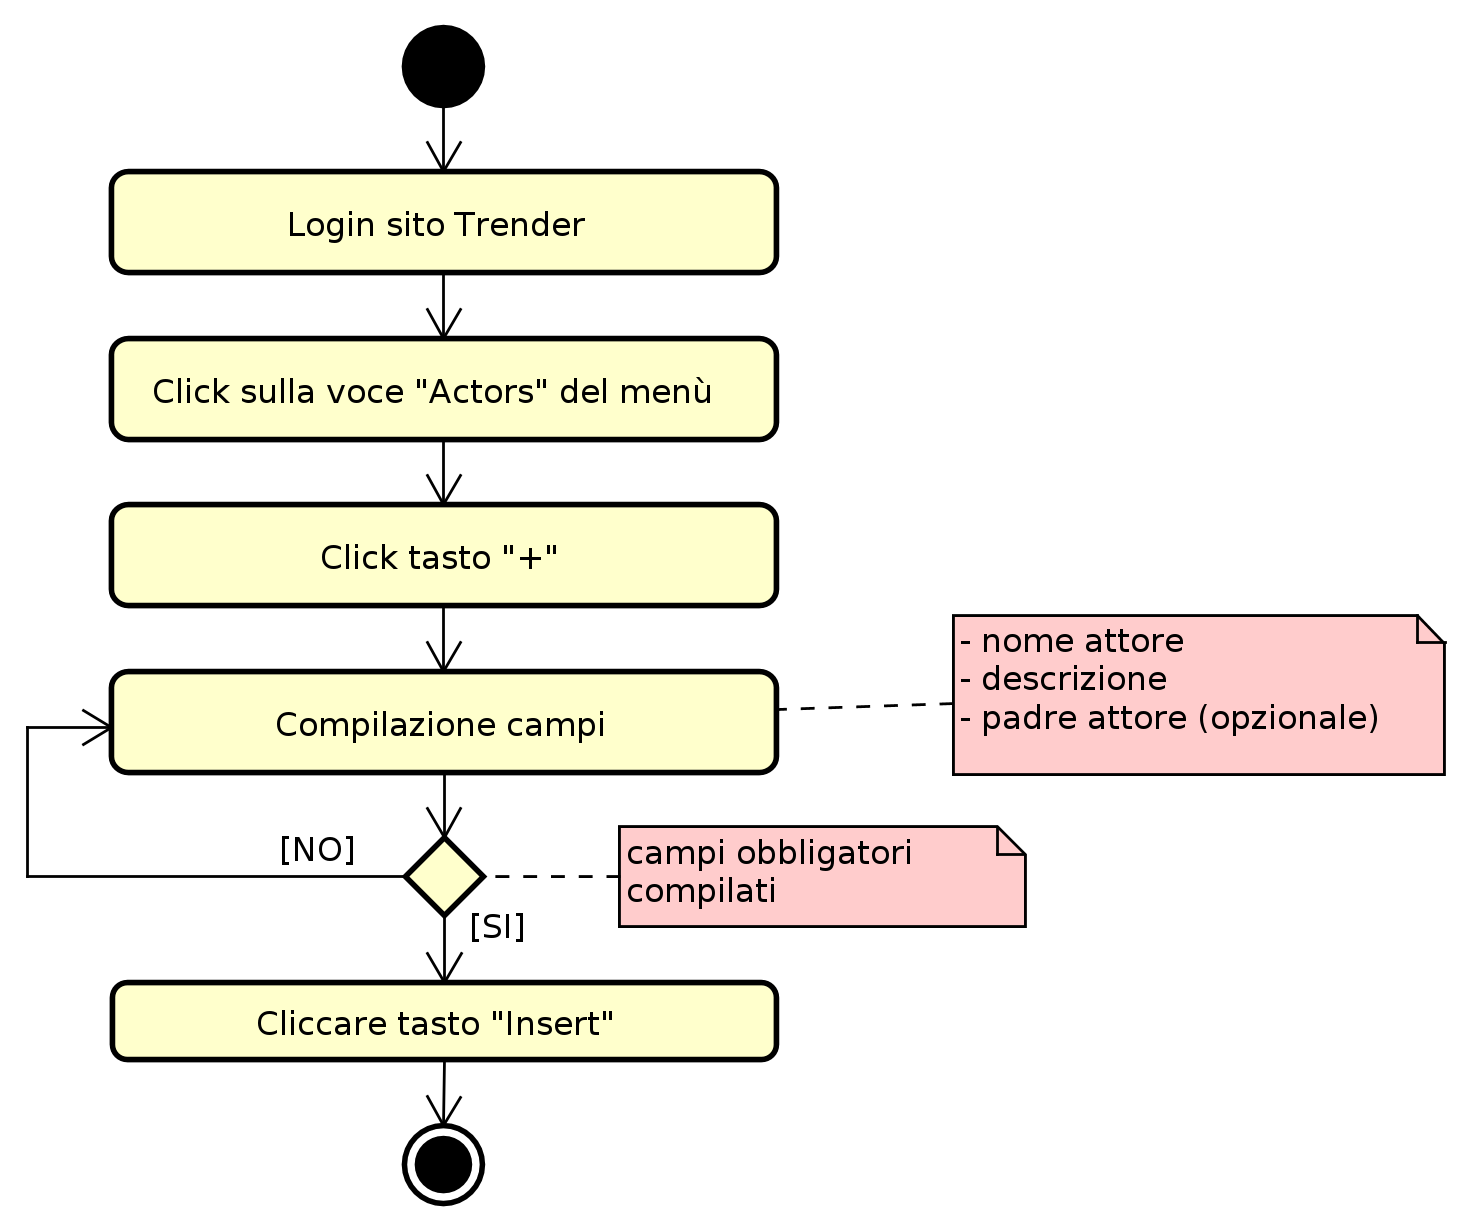
\includegraphics[width=0.7\textwidth]{img/AggiuntaAttore}
	    	\caption{Aggiunta attore.}
	    \end{figure}
	    \paragraph{Modifica ed eliminazione attore su Trender}
	    Questa funzionalità non è stata implementata, pertanto bisogna effettuare la modifica dei campi dati dell'attore o l'eliminazione attraverso l'interfaccia di PhpMyAdmin selezionando la tabella: \texttt{Actors}.
	    
	    \paragraph{Aggiunta use case su Trender}
	    L'aggiunta di uno use case deve rispettare i seguenti passi:
	    \begin{enumerate}
	    	\item login al sito \url{http://zephyrusar.altervista.org/trender/};
	    	\item cliccare sulla voce del menu: \hicode{Usecases};
	    	\item cliccare sul tasto \hicode{+} rosso, in basso a destra;
	    	\item compilare i campi: padre, tipo, titolo, descrizione,  pre-condizione, post-condizione, scenario, estensione, path immagine, didascalia immagine;
	    	\item cliccare sul tasto \hicode{insert}.
	    \end{enumerate}
	    \begin{figure}[H]
	    	\centering
	    	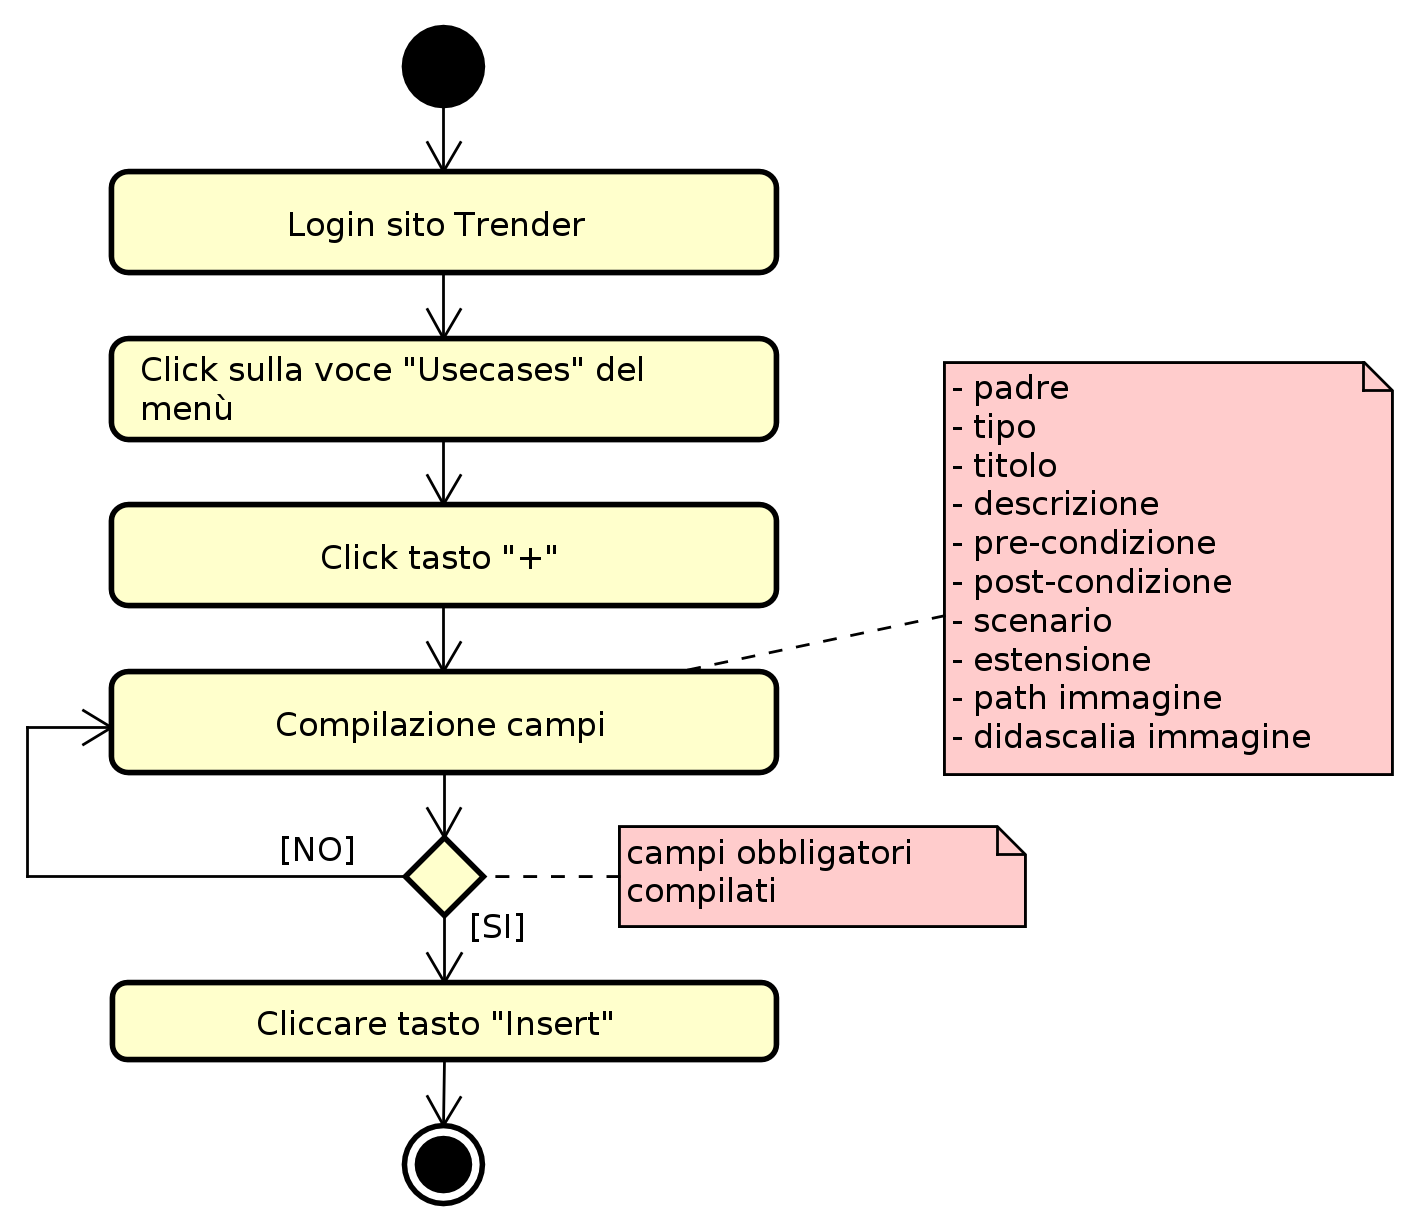
\includegraphics[width=0.7\textwidth]{img/AggiuntaUC}
	    	\caption{Aggiunta use case.}
	    \end{figure}
    
	    \paragraph{Modifica use case su Trender}
	    La modifica di uno use case deve rispettare i seguenti passi:
	    \begin{enumerate}
	    	\item login al sito \url{http://zephyrusar.altervista.org/trender/};
	    	\item cliccare sulla voce del menu: \hicode{Usecases};
	    	\item cliccare sull'\hicode{id} dello use case;
	    	\item modificare i campi: padre, tipo, titolo, descrizione, pre-condizione, post-condizione, scenario, estensione, path immagine, didascalia immagine, associazione use case-attore, associazione use case requisito;
	    	\item cliccare sul tasto \hicode{save}.
	    \end{enumerate}
	    \begin{figure}[H]
	    	\centering
	    	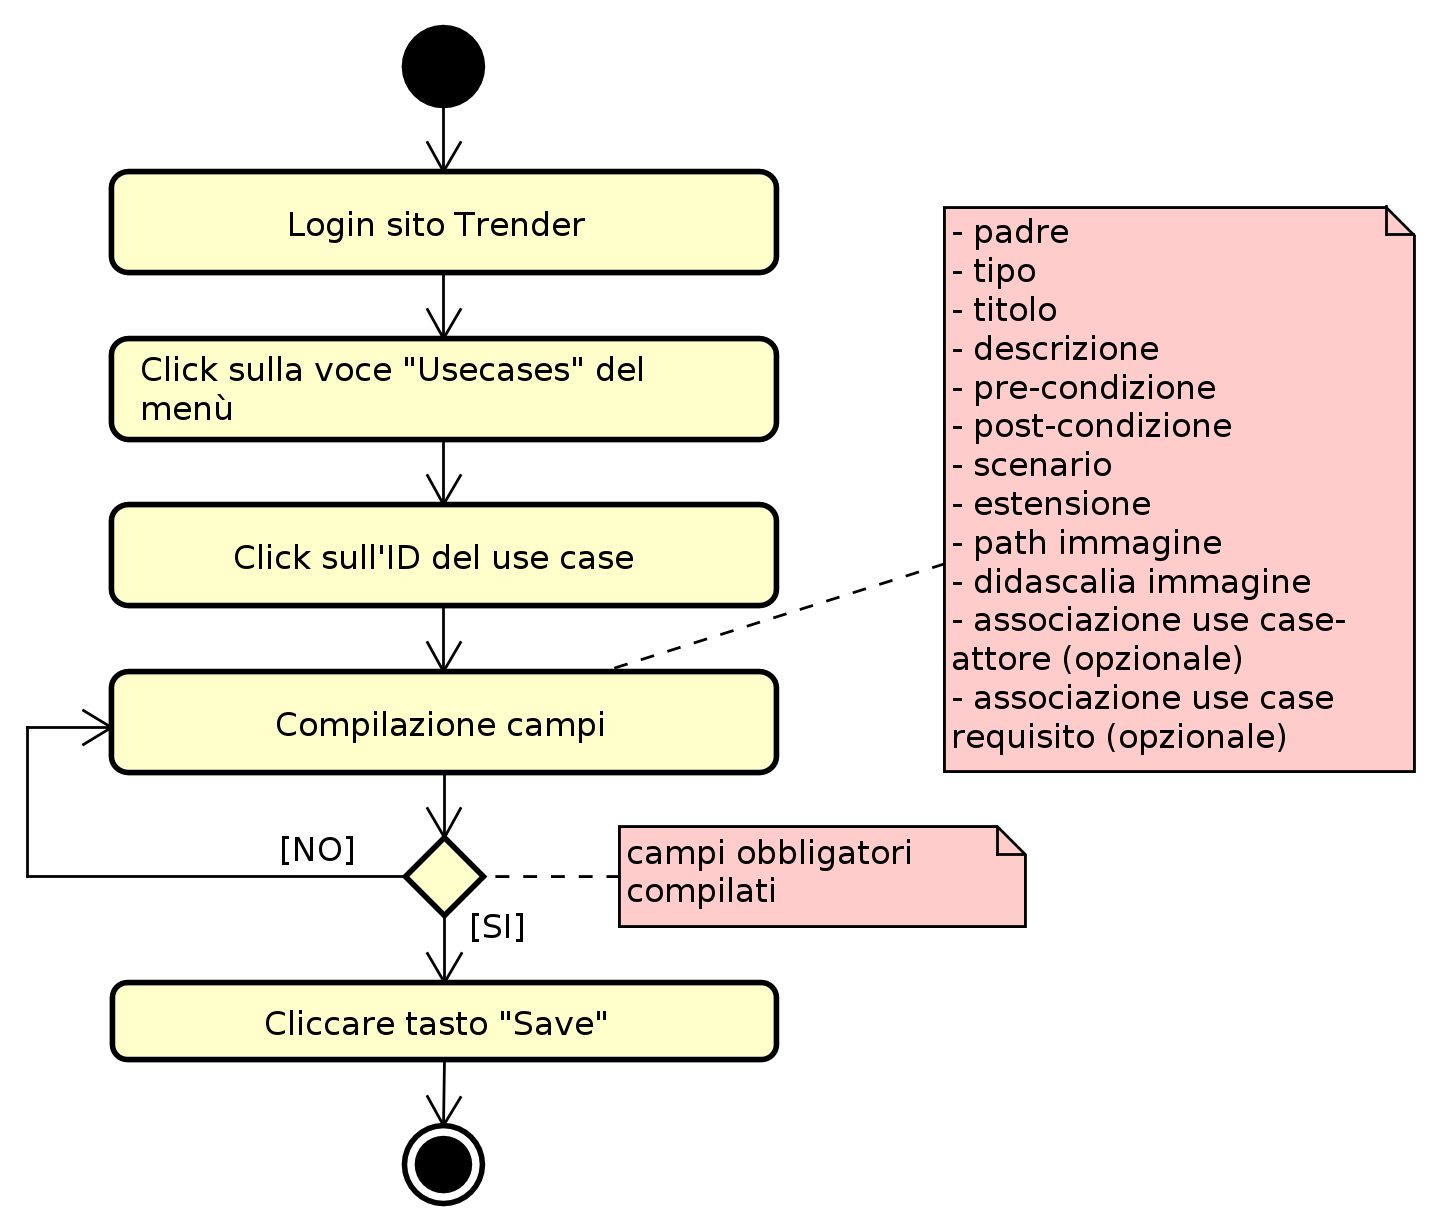
\includegraphics[width=0.7\textwidth]{img/ModificaUC}
	    	\caption{Modifica use case.}
	    \end{figure}
	    
	    \paragraph{Eliminazione use case su Trender}
	    L'eliminazione di uno use case deve rispettare i seguenti passi:
	    \begin{enumerate}
	    	\item login al sito \url{http://zephyrusar.altervista.org/trender/};
	    	\item cliccare sulla voce del menu: \hicode{Usecases};
	    	\item cliccare sull'\hicode{id} dello use case;
	    	\item cliccare sul tasto \hicode{delete use case}.
	    \end{enumerate}

	    \paragraph{Aggiunta requisito su Trender}
	    L'aggiunta di un requisito deve rispettare i seguenti passi:
	    \begin{enumerate}
			\item login al sito \url{http://zephyrusar.altervista.org/trender/};
			\item cliccare sulla voce del menu: \hicode{Requirements};
			\item cliccare sul tasto \hicode{+} rosso, in basso a destra;
			\item compilare i campi: padre, importanza(obbligatorio, desiderabile, facoltativo), tipo(funzionale, prestazionale, qualitativo, vincolo), sorgente, descrizione;
			\item cliccare sul tasto \hicode{insert}.
		\end{enumerate}
		\begin{figure}[H]
			\centering
			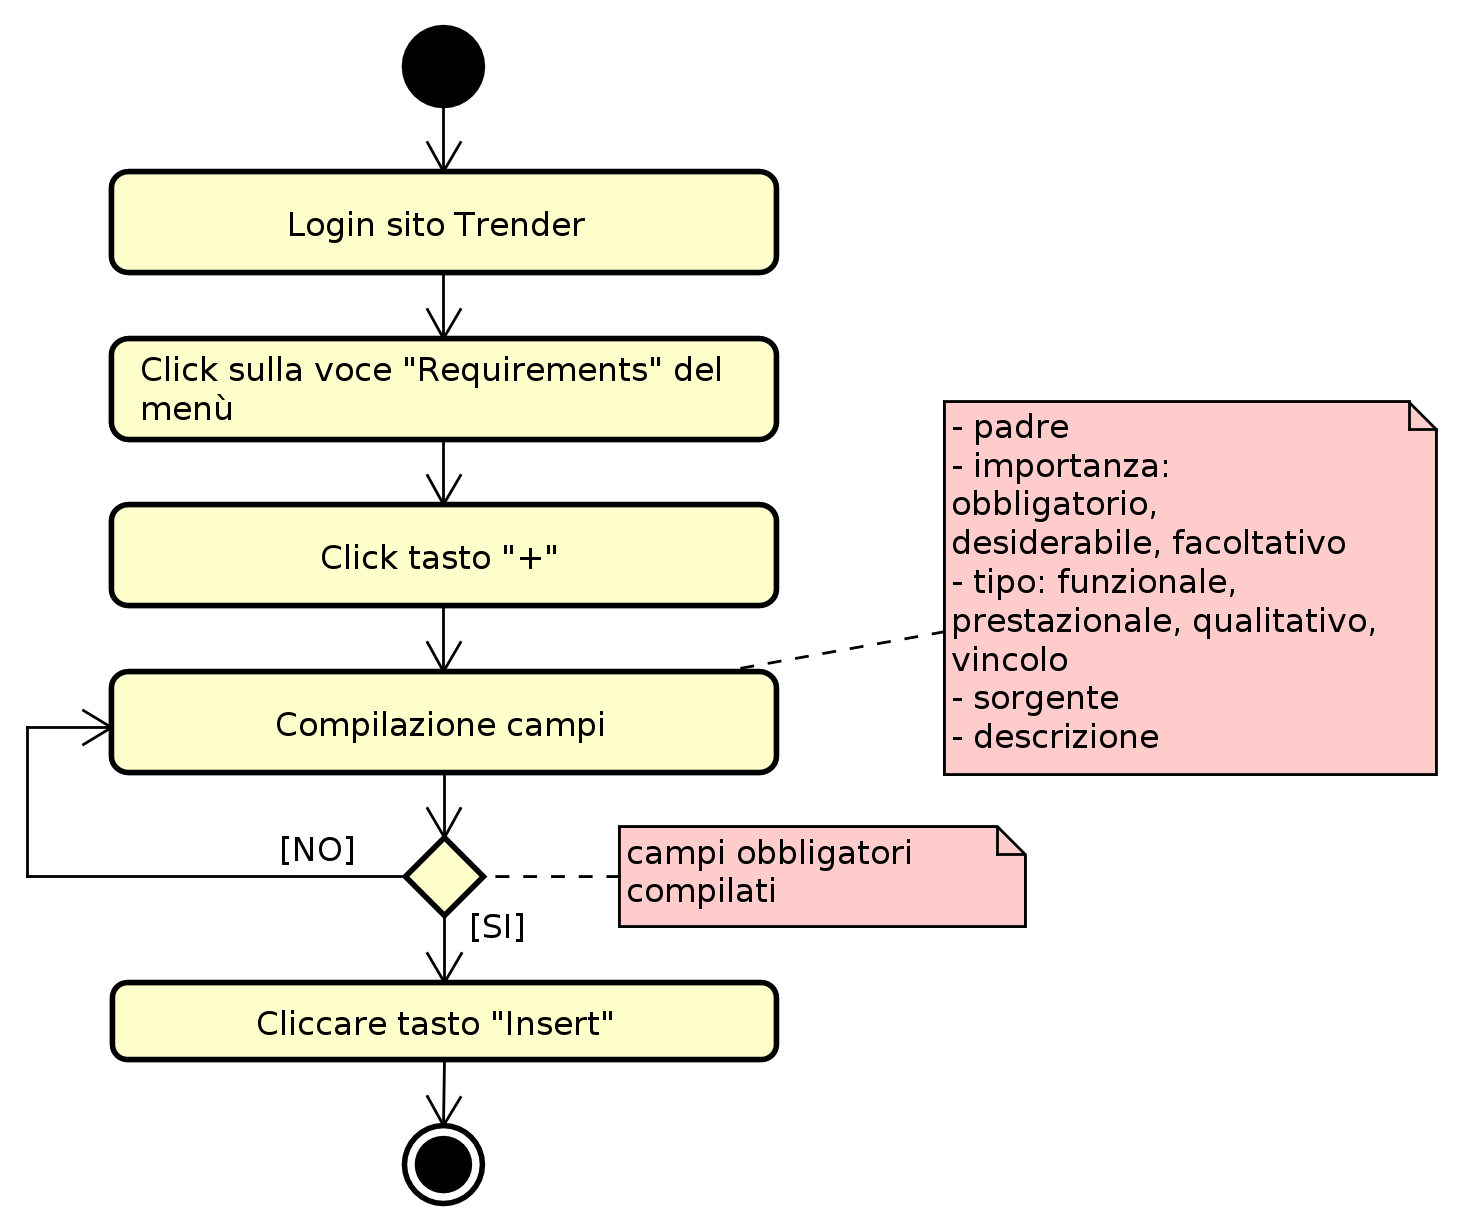
\includegraphics[width=0.7\textwidth]{img/AggiuntaReq}
			\caption{Aggiunta requisito.}
		\end{figure}
			    
		\paragraph{Modifica requisito su Trender}
		La modifica di un requisito deve rispettare i seguenti passi:
		\begin{enumerate}
			\item login al sito \url{http://zephyrusar.altervista.org/trender/};
			\item cliccare sulla voce del menu: \hicode{Requirements};
	    	\item cliccare sull'\hicode{id} del requisito;	
			\item modificare i campi: padre, importanza(obbligatorio, desiderabile, facoltativo), tipo(funzionale, prestazionale, qualitativo, vincolo), sorgente, descrizione, associazione classe (opzionale), package (opzionale), test di sistema (opzionale), test di validazione (opzionale);
			\item cliccare sul tasto \hicode{save}.
		\end{enumerate}
		\begin{figure}[H]
			\centering
			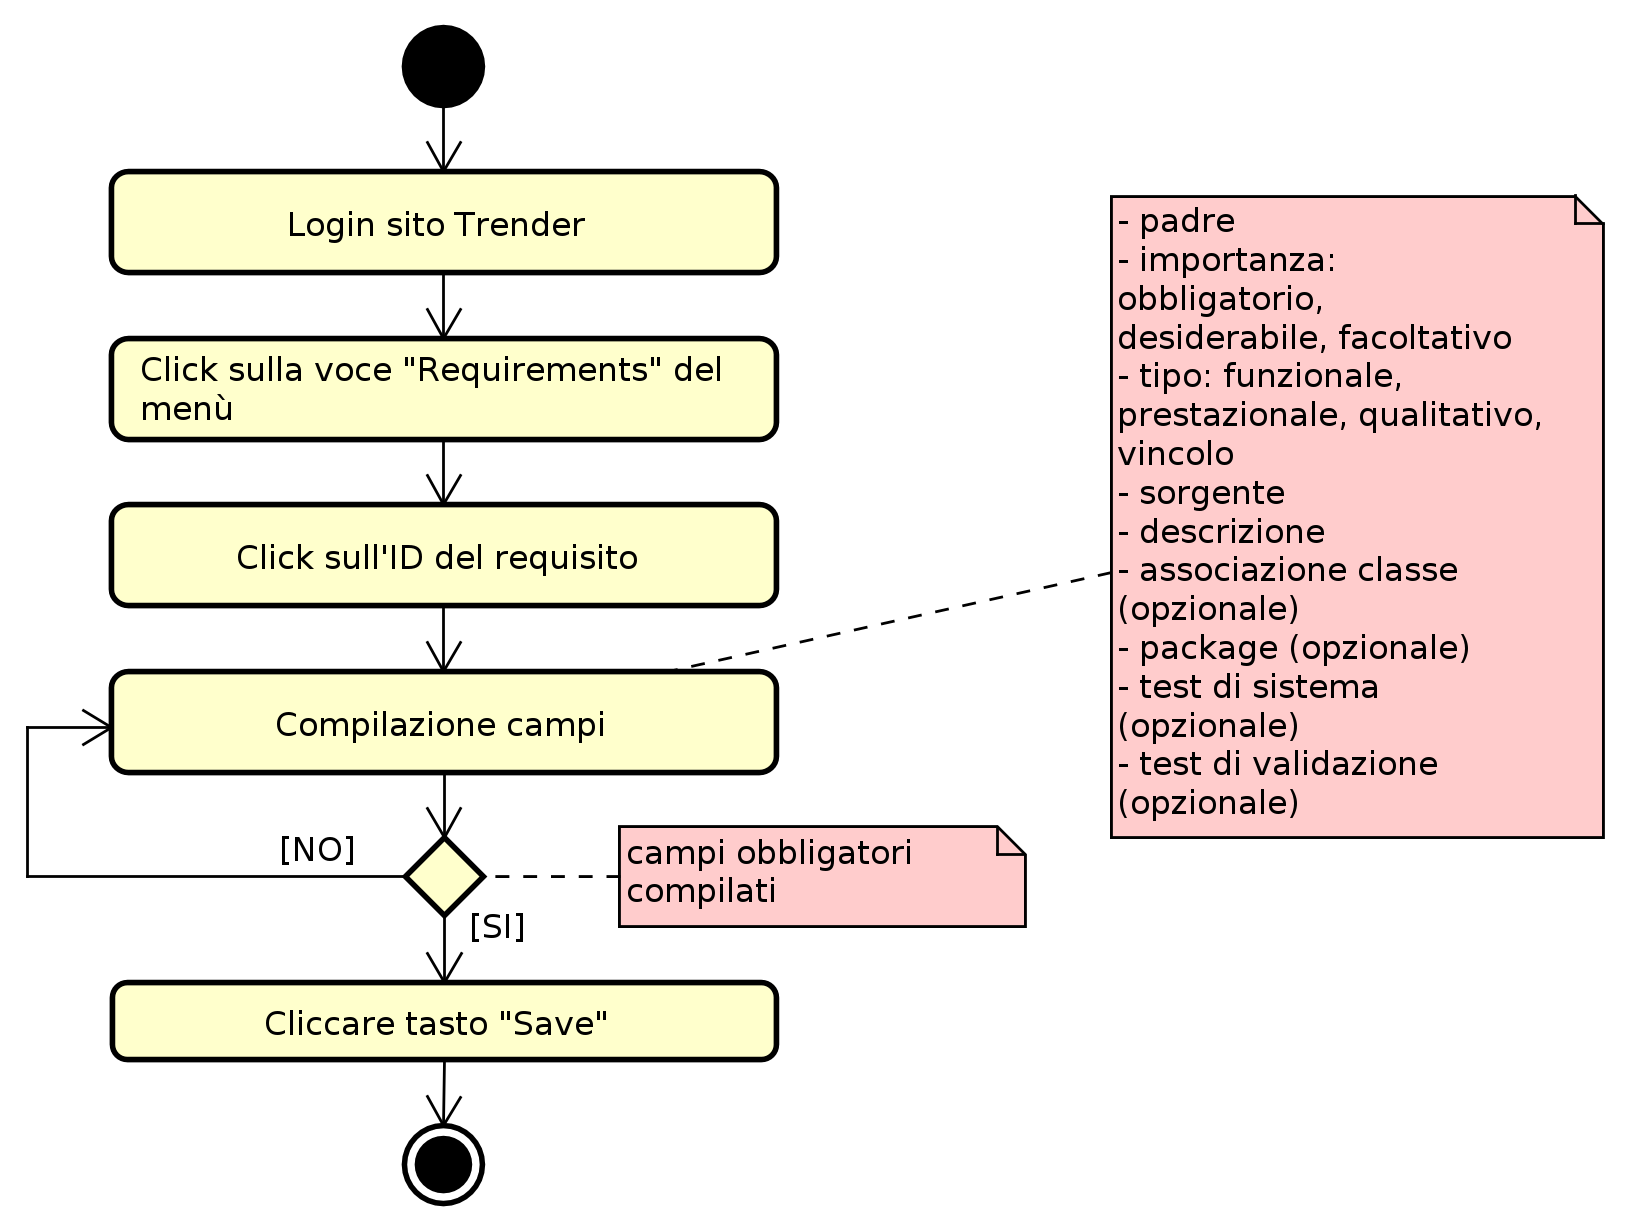
\includegraphics[width=0.7\textwidth]{img/ModificaReq}
			\caption{Modifica requisito.}
		\end{figure}
	
		\paragraph{Eliminazione requisito su Trender}
		L'eliminazione di un requisito deve rispettare i seguenti passi:
		\begin{enumerate}
			\item login al sito \url{http://zephyrusar.altervista.org/trender/};
			\item cliccare sulla voce del menu: \hicode{Requirements};
			\item cliccare sull'\hicode{id} del requisito;
			\item cliccare sul tasto \hicode{delete requirement}.
		\end{enumerate}

		\paragraph{Aggiunta package su Trender} \label{sec:traccComp}
		L'aggiunta di un package deve rispettare i seguenti passi:
		\begin{enumerate}
			\item login al sito \url{http://zephyrusar.altervista.org/trender/};
			\item cliccare sulla voce del menu: \hicode{Packages};
			\item cliccare sul tasto \hicode{+} rosso, in basso a destra;
			\item compilare i campi: nome, descrizione, path immagine, didascalia, padre (opzionale);
			\item cliccare sul tasto \hicode{insert}.
		\end{enumerate}
		\begin{figure}[H]
			\centering
			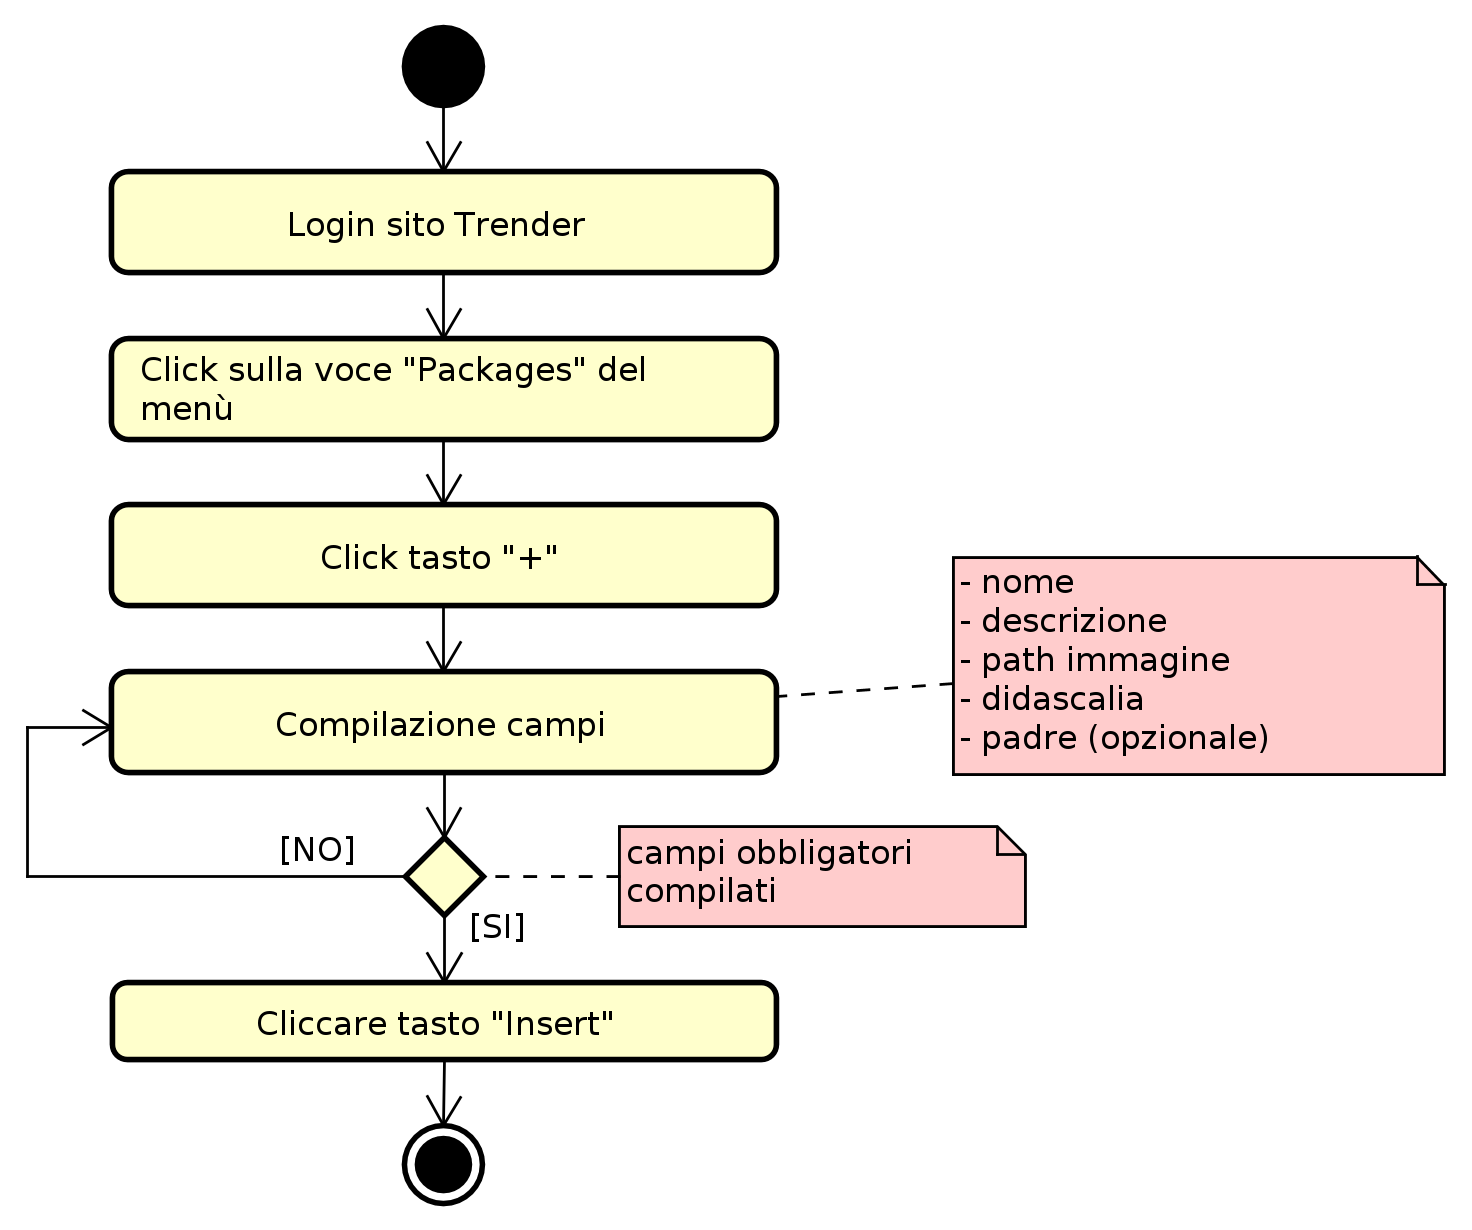
\includegraphics[width=0.7\textwidth]{img/AggiuntaPack}
			\caption{Aggiunta package.}
		\end{figure}
		
		\paragraph{Modifica package su Trender} \label{sec:traccTint}
		La modifica di un package deve rispettare i seguenti passi:
		\begin{enumerate}
			\item login al sito \url{http://zephyrusar.altervista.org/trender/};
			\item cliccare sulla voce del menu: \hicode{Packages};
			\item cliccare sull'\hicode{id} del packages;	
			\item modificare i campi: nome, descrizione, path immagine, didascalia, padre (opzionale), test d'integrazione;
			\item cliccare sul tasto \hicode{save}.
		\end{enumerate}
		\begin{figure}[H]
			\centering
			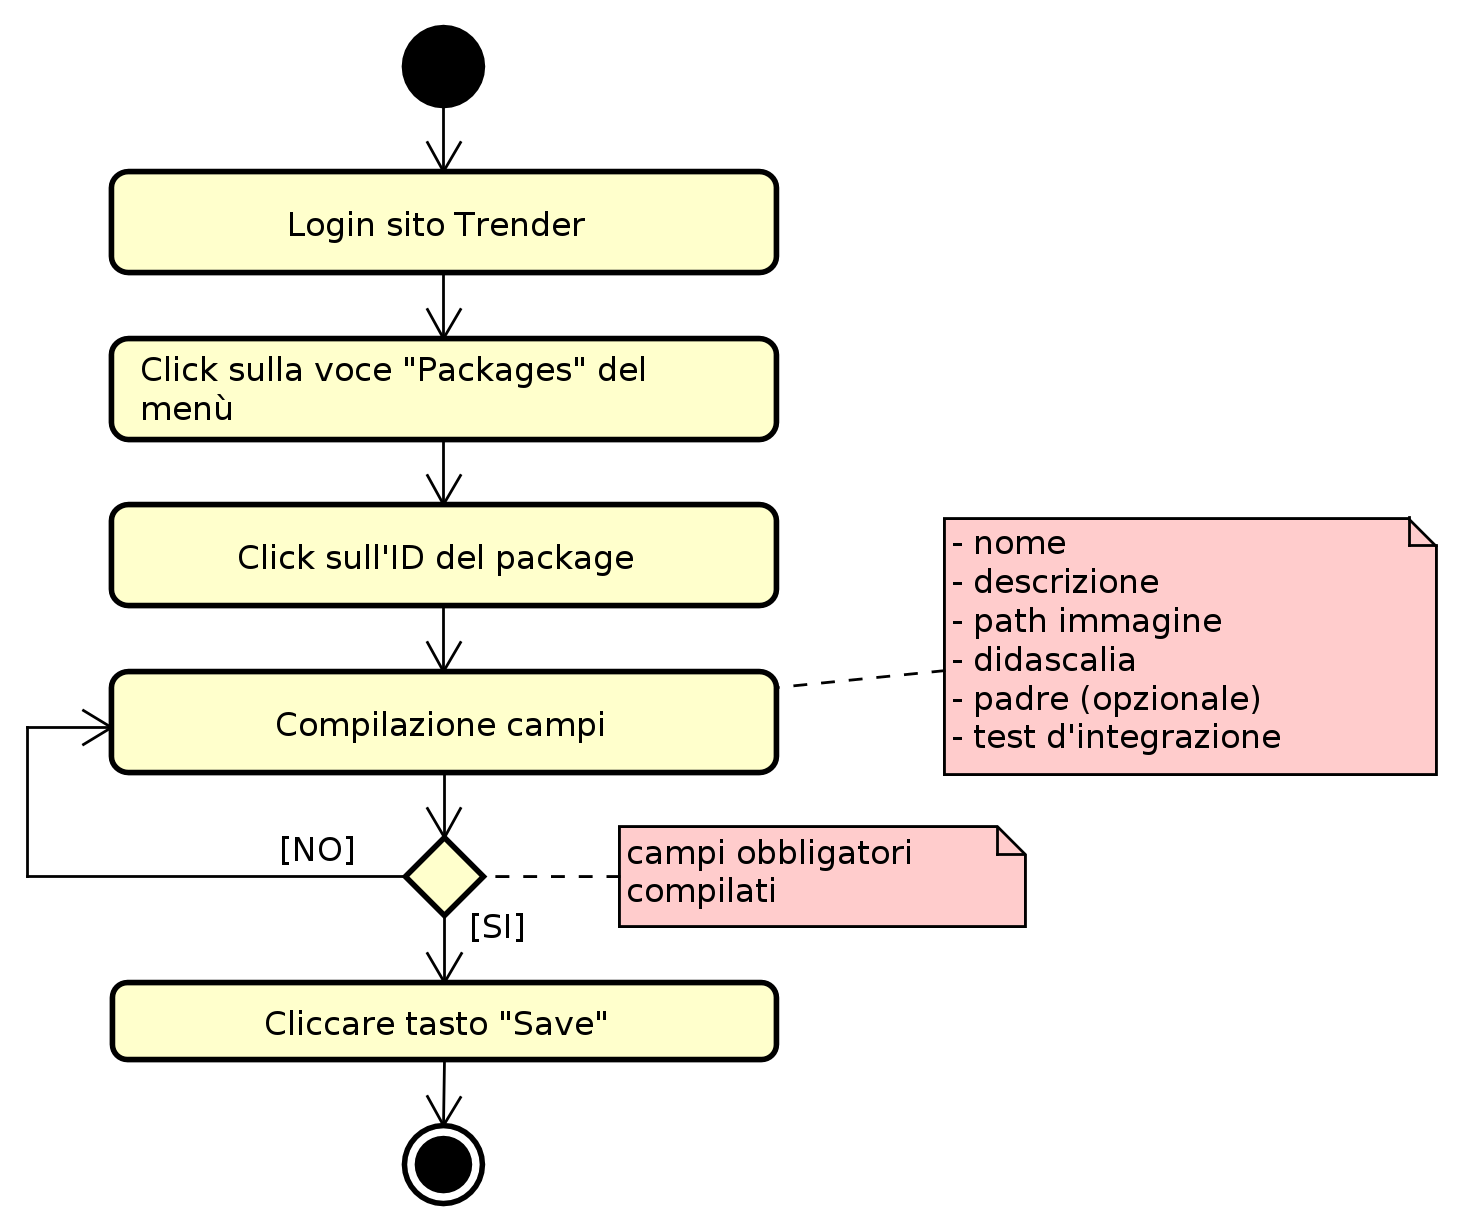
\includegraphics[width=0.7\textwidth]{img/ModificaPack}
			\caption{Modifica package.}
		\end{figure}
	
		\paragraph{Eliminazione package su Trender}				
		L'eliminazione di un package deve rispettare i seguenti passi:
		\begin{enumerate}
			\item login al sito \url{http://zephyrusar.altervista.org/trender/};
			\item cliccare sulla voce del menu: \hicode{Packages};
			\item cliccare sull'\hicode{id} del package;
			\item cliccare sul tasto \hicode{delete package}.
		\end{enumerate}
		
		\paragraph{Aggiunta classe su Trender}
		L'aggiunta di una classe deve rispettare i seguenti passi:
		\begin{enumerate}
			\item login al sito \url{http://zephyrusar.altervista.org/trender/};
			\item cliccare sulla voce del menu: \hicode{Classes};
			\item cliccare sul tasto \hicode{+} rosso, in basso a destra;
			\item compilare i campi: selezione package, nome classe, descrizione, utilizzo;
			\item cliccare sul tasto \hicode{insert}.
		\end{enumerate}
		\begin{figure}[H]
			\centering
			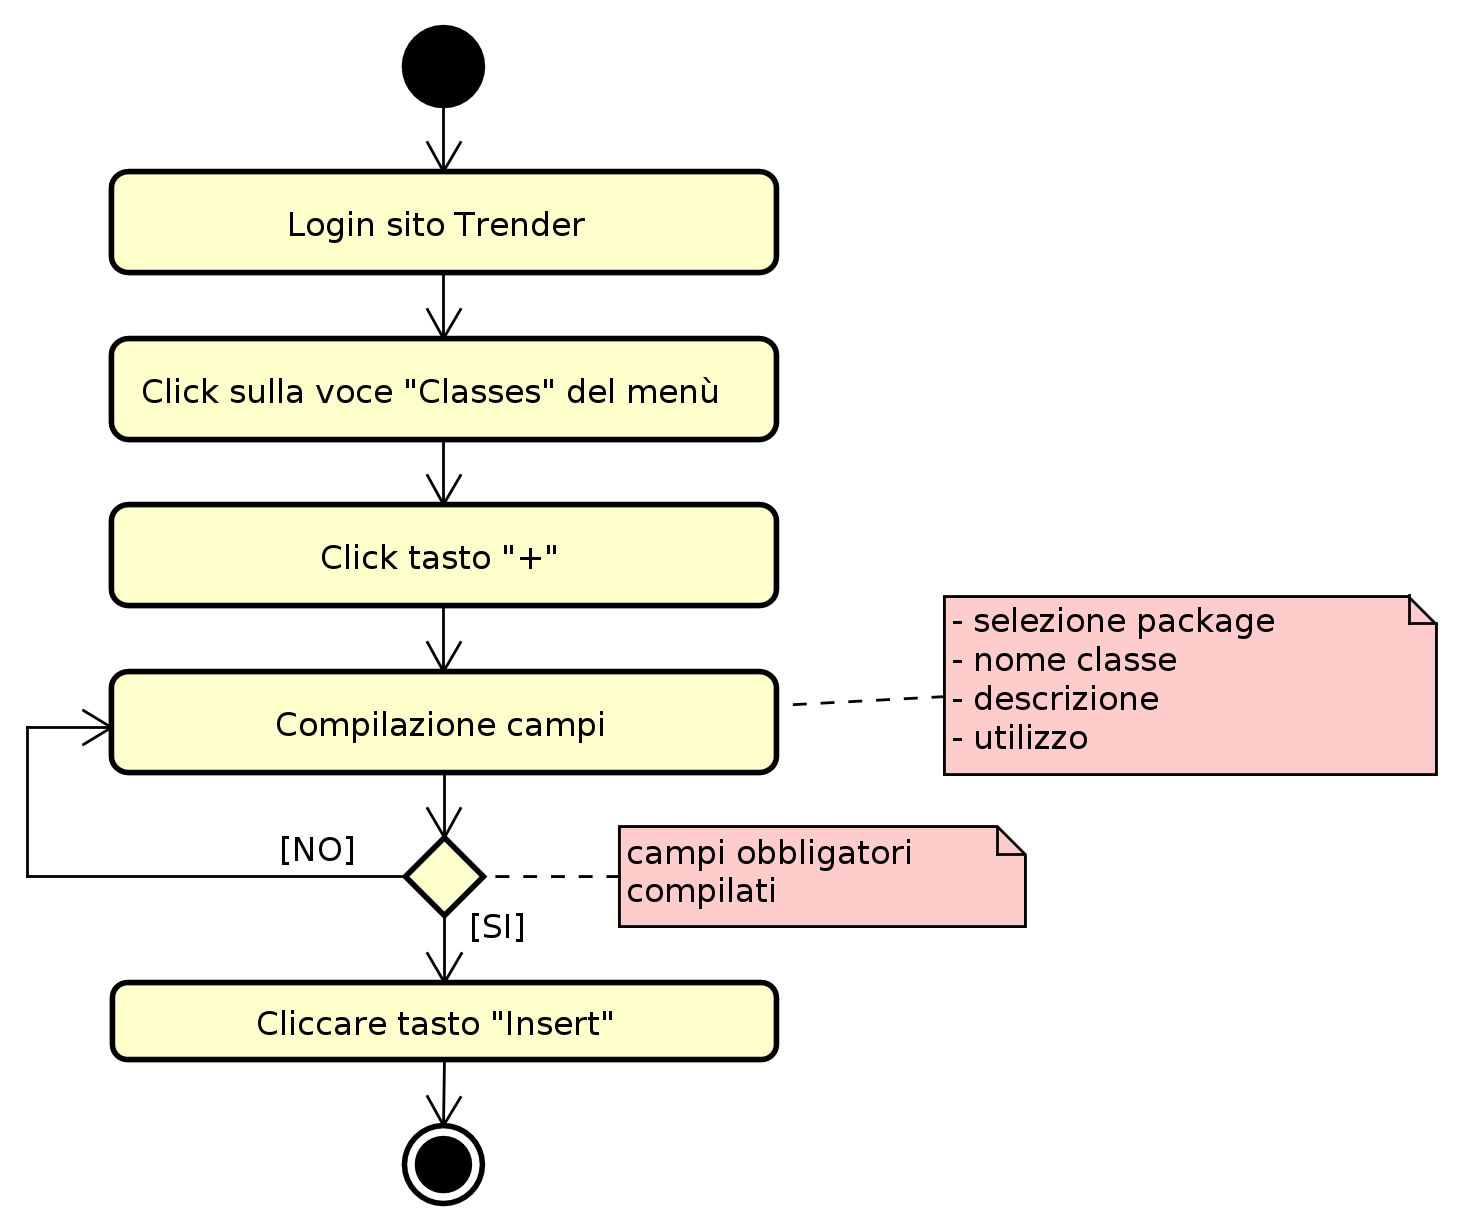
\includegraphics[width=0.7\textwidth]{img/AggiuntaClasse}
			\caption{Aggiunta classe.}
		\end{figure}
		
		\paragraph{Modifica classe su Trender}
		La modifica di una classe deve rispettare i seguenti passi:
		\begin{enumerate}
			\item login al sito \url{http://zephyrusar.altervista.org/trender/};
			\item cliccare sulla voce del menu: \hicode{Classes};
			\item cliccare sull'\hicode{id} della classe;	
			\item modificare i campi: selezione package, nome classe, descrizione, utilizzo, classe base, classe target, tipo relazione, attributi (tipo, nome, descrizione), metodi (tipo di ritorno, segnatura, descrizione, parametri (tipo parametro, nome, descrizione);
			\item cliccare sul tasto \hicode{save}.
		\end{enumerate}
		\begin{figure}[H]
			\centering
			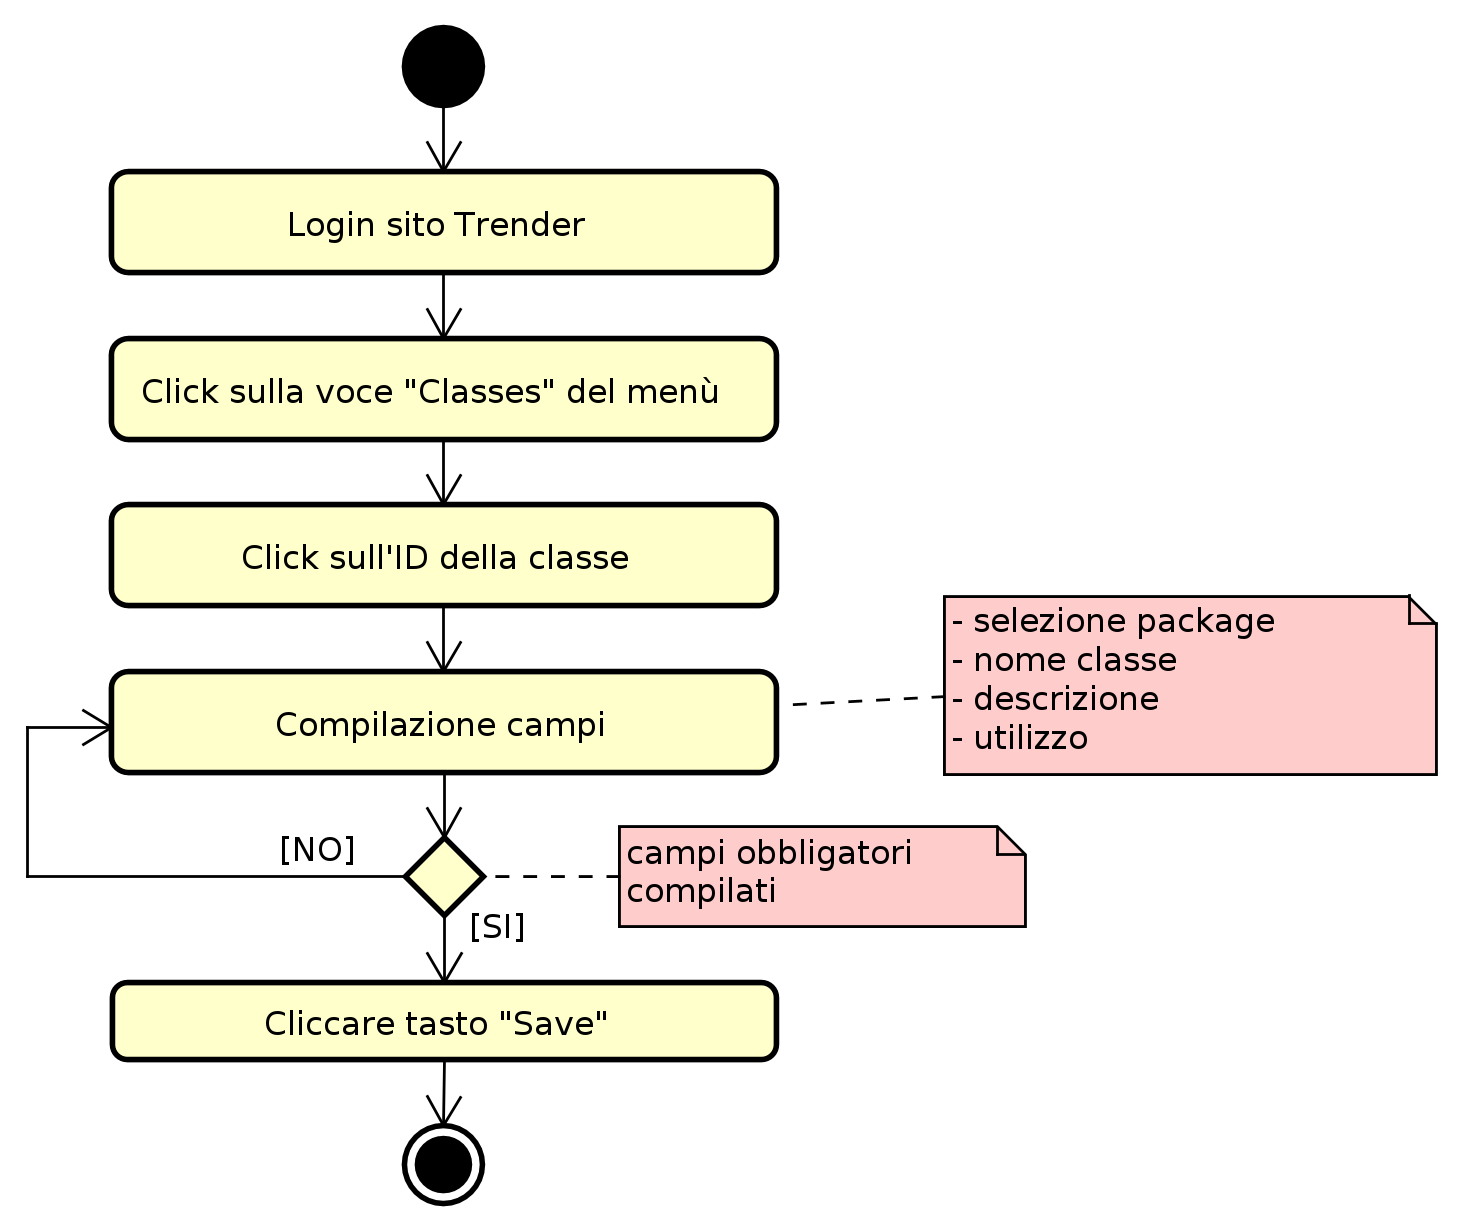
\includegraphics[width=0.7\textwidth]{img/ModificaCl}
			\caption{Modifica classe.}
		\end{figure}
		
		\paragraph{Eliminazione classe su Trender}	
		L'eliminazione di una classe deve rispettare i seguenti passi:
		\begin{enumerate}
			\item login al sito \url{http://zephyrusar.altervista.org/trender/};
			\item cliccare sulla voce del menu: \hicode{Classes};
			\item cliccare sull'\hicode{id} della classe;
			\item cliccare sul tasto \hicode{delete class}.
		\end{enumerate}
		
		\paragraph{Aggiunta test di unità su Trender} \label{sec:traccTuni}
		L'aggiunta di un test di unità deve rispettare i seguenti passi:
		\begin{enumerate}
			\item login al sito \url{http://zephyrusar.altervista.org/trender/};
			\item cliccare sulla voce del menu: \hicode{Test};
			\item cliccare sul tasto \hicode{+} rosso, in basso a destra;
			\item compilare i campi: package, classe, metodo da combinare, descrizione del test;
			\item cliccare sul tasto \hicode{insert}.
		\end{enumerate}
		\begin{figure}[H]
			\centering
			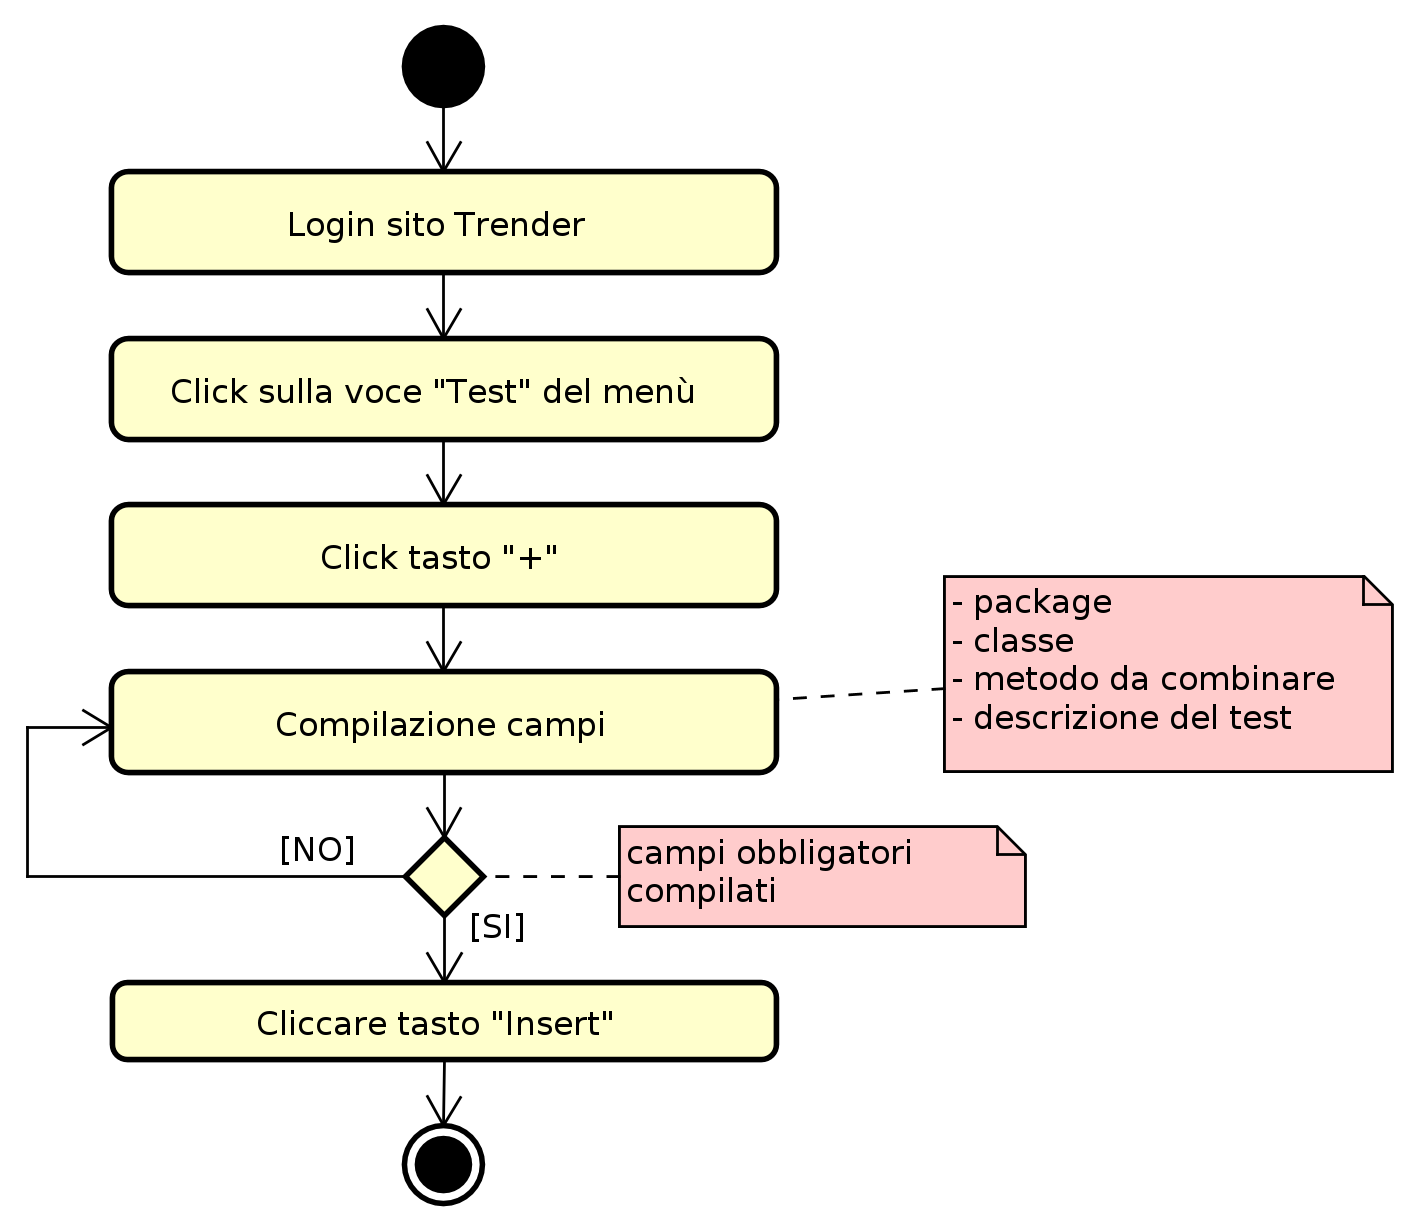
\includegraphics[width=0.7\textwidth]{img/AggiuntaTestUnit}
			\caption{Aggiunta test di unità.}
		\end{figure}

		\paragraph{Modifica ed eliminazione Test di unità su Trender}
		Questa funzionalità non è stata implementata, pertanto bisogna effettuare la modifica dei campi dati del test o l'eliminazione attraverso l'interfaccia di PhpMyAdmin selezionando la tabella: \texttt{UnitTest}.
		%
		\paragraph{Esportazione da Trender a codice \LaTeX}
		L'esportazione del codice \LaTeX{} da Trender deve rispettare i seguenti passi:
		\begin{enumerate}
			\item login al sito \url{http://zephyrusar.altervista.org/trender/};
			\item cliccare sulla voce del menu: \hicode{Prints};
			\item selezionare i campi desiderati per la stampa (di solito tutti);
			\item cliccare sul tasto \hicode{print all};
			\item selezionare la sezione del codice \LaTeX{} da visualizzare;
			\item copiare il codice \LaTeX e incollarlo sul documento desiderato.
		\end{enumerate}
		\begin{figure}[H]
			\centering
			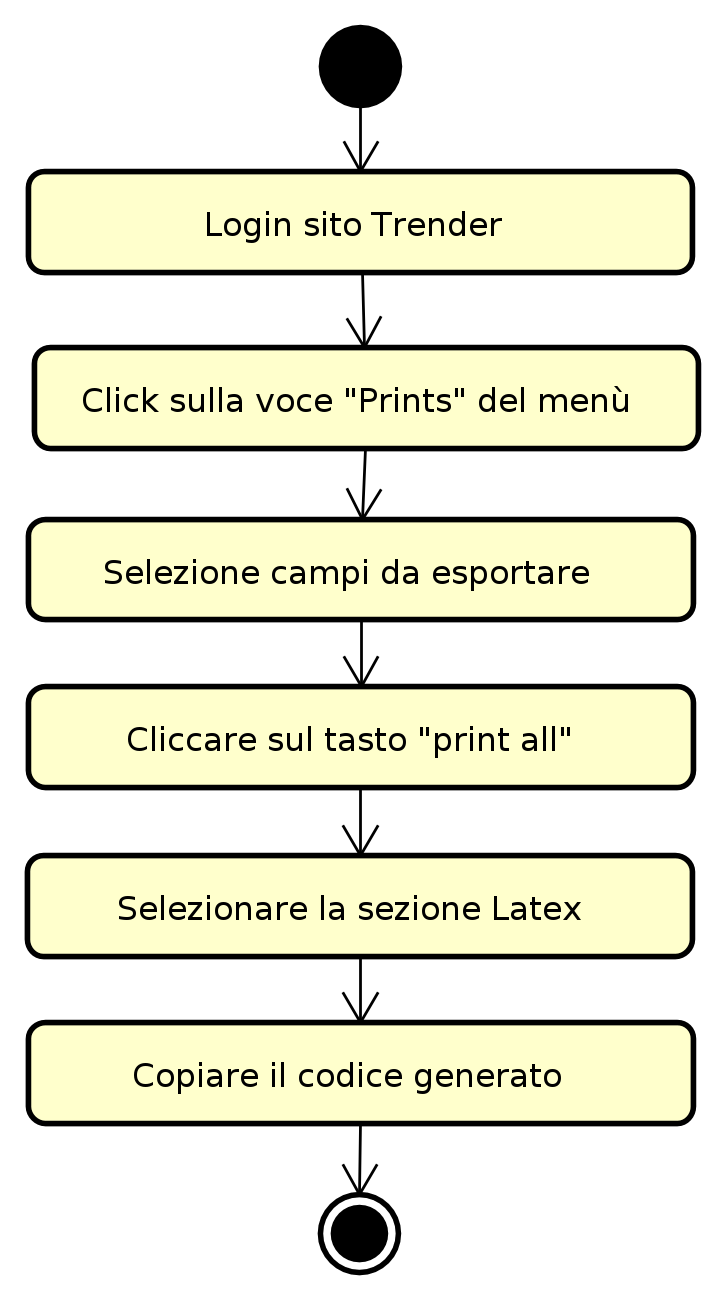
\includegraphics[width=0.3\textwidth]{img/Export}
			\caption{Esportazione codice \LaTeX{} da Trender.}
		\end{figure}
		%
		\paragraph{Impostazioni Trender}
		Alcune impostazioni di Trender si possono modificare rispettando i seguenti passi:
		\begin{enumerate}
			\item login al sito \url{http://zephyrusar.altervista.org/trender/};
			\item cliccare sulla voce del menu a forma di ingranaggio;
			\item inserire la sorgente dei requisiti: nome sorgente.
		\end{enumerate}
		%
		\paragraph{Configurazione WebStorm}
		Lo stile di codifica adottato (vedi sezione \ref{codeStyle}) e personalizzato per questo progetto deve essere importato all'interno di WebStorm nel tool ESLint. Per fare questo è necessario seguire i seguenti passaggi:
		\begin{enumerate}
			\item aprire WebStorm;
			\item aprire il menu \hicode{File -> Preferences};
			\item entrare nel menu \hicode{Language \& Frameworks->JavaScript->Code Quality Tools->ESLint};
			\item abilitare il tool essicurandosi di aver installato prima Node.js (vedi sezione \ref{nodejs});
			\item selezionare nel campo ESLint package il file che si trova all'interno del progetto \hicode{DeGeOp/node\_modules/eslint};
			\item salvare le impostazioni premendo il tasto \hicode{Ok}.
		\end{enumerate}
		

